\documentclass[12pt,a4paper]{report} % Classe de document pour un rapport avec une taille de police de 12 points

% Encodage et langue
\usepackage[utf8]{inputenc} % Permet d'utiliser les accents
\usepackage[T1]{fontenc}
\usepackage[english]{babel} % Définit le français comme langue principale
\usepackage{amsmath}
\usepackage{listings}
\usepackage{stmaryrd}
\usepackage{titlesec}

\titleformat{\chapter}[display]
  {\normalfont\LARGE\bfseries} % Style du titre
  {}                          % Pas de numéro de chapitre
  {0pt}                       % Espace entre le numéro et le titre
  {\LARGE}                    % Taille du titre
  
% Marges et mise en page
\usepackage{geometry}
\geometry{left=2.5cm, right=2.5cm, top=3cm, bottom=3cm}

% Liens cliquables pour la table des matières
\usepackage{hyperref}
\hypersetup{
    colorlinks=true,
    linkcolor=blue,
    urlcolor=blue,
    pdftitle={Summative Assignment COMPOO86},
    pdfauthor={Benoît Coutière}
}

% Pour insérer des graphiques
\usepackage{graphicx}
\usepackage{float}

% Pour faire des tableaux plus jolis
\usepackage{array}
\usepackage{booktabs}

% Début du document
\begin{document}

% Page de titre
\begin{titlepage}
    \centering
    {\scshape\LARGE MSc in Machine Learning - 2024/2025 \par}
    \vspace{4cm}
    {\scshape\Large Summative Assignment of \par}
    \vspace{0.5cm}
    {\huge\bfseries Probabilistic and Unsupervised Learning\par}
    \vspace{4cm}
    {\LARGE Benoît Coutière \par}
    \vfill
    
\includegraphics[width=1\textwidth]{images/University_College_London_logo.svg.png}
    \vfill

\end{titlepage}

% Page de garde pour la table des matières
\pagenumbering{roman} % Numérotation des pages en chiffres romains pour les préliminaires
\tableofcontents
\newpage
\listoffigures % Si tu as des figures
\listoftables % Si tu as des tableaux
\newpage

\pagenumbering{arabic} % Numérotation des pages en chiffres arabes pour le corps principal

% Section 1
\chapter{Exercise 1}
\item a)
Since the multivariate Gaussian is a probability density modeling variables which can take any continuous values, this is not appropriate to model our discrete problem.\\

\item b)
We have:
\[
arg \max_p \left( P(x|p) \right) = arg \max_p \left( \log(P(x|p)) \right)
\]

All \( x^{(n)} \) are mutually independent, so we have:
\[
P(X|p) = \prod_{n=1}^{N} P(x^{(n)}|p) = \prod_{n=1}^{N} \prod_{d=1}^{D} p_d^{x_d^{(n)}} (1-p_d)^{1-x_d^{(n)}}
\]

Thus:
\[
\log(P(x|p)) = \sum_{n=1}^{N} \sum_{d=1}^{D} x_d^{(n)} \log(p_d) + (1-x_d^{(n)}) \log(1-p_d)
\]

If we denote \( p^* \) as the solution of \( arg \max_p \left( \log(P(x|p)) \right) \), we have :
\[
\frac{\partial}{\partial p_i} \left( \sum_{n=1}^{N} \sum_{d=1}^{D} x_d^{(n)} \log(p_d) + (1-x_d^{(n)}) \log(1-p_d) \right) = 0,\forall i \in [1; D], i \in \mathbb{N}
\]

\[
\implies \sum_{n=1}^{N} \frac{x_i^{(n)}}{p_i^*} - \frac{1-x_i^{(n)}}{1-p_i^*} = 0
\]

\[
\implies \frac{A_i}{p_i^*} - \frac{N-A_i}{1 - p_i^*} = 0, \quad \text{with} \quad A_i = \sum_{n=1}^{N} x_i^{(n)}
\]

\[
\implies \forall i \in \llbracket1; D\rrbracket, p_i^* = \frac{A_i}{N}
\]

Finally, we have:
\[
p^* = \begin{bmatrix}
\frac{1}{N} \sum_{n=1}^{N} x_1^{(n)} \\
\vdots \\
\frac{1}{N} \sum_{n=1}^{N} x_D^{(n)} \\
\end{bmatrix}
\]

\item c)

We have:
\[
p_{MAP} = arg \max_p \left( P(p | (x^{(1)}, \dots, x^{(n)})) \right)
\]

Using Bayes' Rule, we obtain:
\[
p_{MAP} = arg \max_p \left( \frac{P(p) P((x^{(1)}, \dots, x^{(n)}) | p)}{P((x^{(1)}, \dots, x^{(n)}))} \right)
\]

Since \( P((x^{(1)}, \dots, x^{(n)})) \) is independent from \( p \), we have:
\[
p_{MAP} = arg \max_p \left( P(p) P((x^{(1)}, \dots, x^{(n)}) | p) \right)
\]

Given that \( (x^{(1)}, \dots, x^{(n)}) \) are iid, we get:
\[
p_{MAP} = arg\max_p \left( P(p) \prod_{n=1}^{N} P(x^{(n)} | p) \right)
\]
\[
= arg\max_p \left( \log(P(p)) + \sum_{n=1}^{N} \log(P(x^{(n)} | p)) \right)
\]

Thus, \( (p_{MAP})_i \) is given by:
\[
\frac{\partial}{\partial p_i} \left( \log(P(p)) + \sum_{n=1}^{N} \log(P(x^{(n)} | p)) \right) = 0
\]

\[
\implies \frac{\partial}{\partial p_i} \left( \log\left( \frac{p_i^{\alpha-1}(1-p_i)^{\beta-1}}{B(\alpha, \beta)} \right) + \sum_{n=1}^{N} \log(P(x^{(n)} | p)) \right) = 0 \]
with $p_i\neq$ 0 and $p_i\neq$ 1


\[
\implies \frac{(\alpha - 1)}{p_i} - \frac{\beta - 1}{1 - p_i} + \sum_{n=1}^{N} \sum_{d=1}^{D} \frac{\partial}{\partial p_i} \log \left( p_d^{x_d^{(n)}} (1-p_d)^{1-x_d^{(n)}} \right) = 0
\]


\[
\implies \frac{(\alpha - 1)(1 - p_i) - (\beta - 1)p_i + (1 - p_i)A_i - Np_i + A_ip_i}{p_i(1 - p_i)} = 0, \quad \text{with} \quad A_i = \sum_{n=1}^{N} x_i^{(n)}
\]

\[
\implies \forall i \in \llbracket 1; D \rrbracket, \quad p_i = - \frac{\alpha - 1 + A_i}{2 - \alpha - \beta - N}
\]

Finally:
\[
p_{MAP} = \begin{bmatrix}
- \frac{\alpha - 1 + \sum_{n=1}^{N} x_1^{(n)}}{2 - \alpha - \beta - N} \\
\vdots \\
- \frac{\alpha - 1 + \sum_{n=1}^{N} x_D^{(n)}}{2 - \alpha - \beta - N}
\end{bmatrix}
\]

\item d)

Here is the code I implemented using python, and the resulting image : 

\begin{lstlisting}[language=Python, basicstyle=\ttfamily\small, frame=single, breaklines=true]
#We load the dataset
X = np.loadtxt('binarydigits.txt')

#We compute the ML parameters
def ML_parameters(input):
    N, D = input.shape
    p=np.zeros(shape=D)
    for d in range (D):
        pd=0
        for n in range (N):
            pd+=input[n,d]
        p[d]=pd/N
    return p 

#We print the numerical result
print(ML_parameters(X).reshape((8,8)))

#We print the resulting image
plt.figure()
plt.imshow(np.reshape(ML_parameters(X), (8,8)),
           interpolation="None",cmap='gray')
plt.axis('off')
\end{lstlisting}

\begin{figure}[h!] % Position de l'image : 'h!' tente de placer l'image ici
    \centering % Centrage de l'image
    
\includegraphics[width=0.5\textwidth]{images/image_1d.png}
    \caption{Visualization of the learned ML parameter vector as an image} % Légende sous l'image
    \label{fig:image1} % Étiquette pour faire référence à l'image dans le texte
\end{figure}

\item e)

You will find below the code I implemented, and the resulting image. We can see that the result obtained is quite similar to the one we had with the ML estimate. We can deduce that our priors are not very useful, and we might consider investigating other prior distributions that would represent better the behavior of $p_d$ than a Beta distribution. If we do not have any better prior available, we could stay with the ML estimate, as it's computationally lighter.

\begin{lstlisting}[language=Python, basicstyle=\ttfamily\small, frame=single, breaklines=true]

#We load the dataset
X = np.loadtxt('binarydigits.txt')

#We compute the MAP parameters
def MAP_parameters(input, alpha=3, beta=3):
    N, D = input.shape
    P=np.zeros(shape=D)
    for d in range (D):
        Pd=0
        for n in range (N):
            Pd+=input[n,d]
        P[d]=(-alpha+1-Pd)/(2-alpha-beta-N)
        #print(Pd/N, P[d])
    return P

#We print the resulting image
plt.figure()
plt.imshow(np.reshape(MAP_parameters(X), (8,8)),
           interpolation="None",cmap='gray')
plt.axis('off')

\end{lstlisting}

\begin{figure}[h!] % Position de l'image : 'h!' tente de placer l'image ici
    \centering % Centrage de l'image
    
\includegraphics[width=0.5\textwidth]{images/image_1e.png}
    \caption{Visualization of the learned MAP parameter vector as an image} % Légende sous l'image
    \label{fig:image1} % Étiquette pour faire référence à l'image dans le texte
\end{figure}





% Section 2
\chapter{Exercise 2}

We will first compute the likelihoods of each of the three models.\\

\item \underline{\textbf{First Model}} \\

For the first model, we will express P(X|p=[$\frac{1}{2}, ...,\frac{1}{2}]^T)$

\[
P(X|p=[\frac{1}{2}, ...,\frac{1}{2}]^T) = \Pi_{n=1}^N \Pi_{d=1}^D (\frac{1}{2})^{x_d^{(n)}} (\frac{1}{2})^{1-x_d^{(n)}} = (\frac{1}{2})^{ND}
\]\\

\item \underline{\textbf{Second Model}} \\

For the second model, we will express P(X|p=[$p, ...,p]^T)$, with p $\in ]0,1[$. We therefore need to "sum" the formula given in the problem statement over all the possible values of p.

\[
 P(X|p=[p, ...,p]^T) = \int_0^1 \Pi_{n=1}^N \Pi_{d=1}^D (p)^{x_d^{(n)}} (1-p)^{1-x_d^{(n)}} dp
\]\\

\[ \implies
 P(X|p=[p, ...,p]^T) = \int_0^1  (p)^{\sum_{n=1}^N \sum_{d=1}^Dx_d^{(n)}} (1-p)^{\sum_{n=1}^N \sum_{d=1}^D (1-x_d^{(n)})} dp
\]\\

If we note A=$\sum_{n=1}^N \sum_{d=1}^Dx_d^{(n)}$, we obtain the following expression:\\ 
\[ 
 P(X|p=[p, ...,p]^T) = \int_0^1  (p)^{A} (1-p)^{(ND-A)}} dp
\]\\

We recognize here a Beta distribution, hence : \\

\[ 
 P(X|p=[p, ...,p]^T) = B(A+1, DN-A+1) = \frac{(A)! (DN-A)!}{(DN+1)!}
\]\\

\item \underline{\textbf{Third Model}} \\

For the third model, we will express P(X|p=[$p_1, ...,p_D]^T)$, with $(p_i)_{i \in \llbracket 1, D \rrbracket \}$ $\in ]0,1[$. We therefore need to "sum" the formula given in the problem statement over all the possible values of $p_i$.

\[
 P(X|p=[p_1, ...,p_D]^T) = \int_0^1 ... \int_0^1 \Pi_{n=1}^N \Pi_{d=1}^D (p)^{x_d^{(n)}} (1-p)^{1-x_d^{(n)}} dp_1...dp_D
\]\\

\[ \implies
 P(X|p=[p_1, ...,p_D]^T) = 
 \] 
\[ \int_0^1 ... \int_0^1 \Pi_{n=1}^N \Pi_{d=1}^D (p)^{x_d^{(n)}} (1-p)^{1-x_d^{(n)}} (\int_0^1 \Pi_{n=1}^N \Pi_{d=1}^D (p)^{x_d^{(n)}} (1-p)^{1-x_d^{(n)}}dp_1) dp_2...dp_D
\]\\

\[ \implies
 P(X|p=[p_1, ...,p_D]^T) = 
 \] 
\[ \int_0^1 ... \int_0^1 \Pi_{n=1}^N \Pi_{d=1}^D (p)^{x_d^{(n)}} (1-p)^{1-x_d^{(n)}} (B(\alpha_1+1, N-\alpha_1+1)) dp_2...dp_D
\]

\begin{center}
with $\alpha_1 = \sum_{n=1}^N x_1^{(n)}$
\end{center}


\[ \implies
 P(X|p=[p_1, ...,p_D]^T) = \Pi_{d=1}^D B(\alpha_d+1, N-\alpha_d+1)
 \]

 \begin{center}
with $\alpha_d = \sum_{n=1}^N x_d^{(n)}$
\end{center}

\[ \implies
 P(X|p=[p_1, ...,p_D]^T) = \frac{\Pi_{d=1}^D (\alpha_d)!(N-\alpha_d)!}{((N-1)!)^D}
 \]

 \item \underline{\textbf{Relative probabilities}} \\

Let's note Mod1, Mod2 and Mod3 our three models. \\

Thanks to Bayes theorem, we have that $\forall k \in \llbracket 1, 3 \rrbracket, p(Mod_k|X)=\frac{P(X|Mod_k)P(Mod_k)}{P(X)}$.\\

We know that $\forall k \in \llbracket 1, 3 \rrbracket,  P(Mod_k)= \frac{1}{3}$. \\

We also know that $P(X) = \sum_{k=1}^3 P(Mod_k) P(X|Mod_k)$.= \sum_{k=1}^3 \frac{1}{3} P(X|Mod_k)$. \\

Finally, we have $\forall k \in \llbracket 1, 3 \rrbracket, p(Mod_k|X)=\frac{P(X|Mod_k)\frac{1}{3}}{\sum_{k=1}^3 \frac{1}{3} P(X|Mod_k)} = \frac{P(X|Mod_k)}{\sum_{k=1}^3 P(X|Mod_k)} $

 \item \underline{\textbf{Code and results}} \\

To compute the probabilities of our 3 models, we used the code below. To avoid having problems of overfloat/underfloat, we worked with log10 and used the Decimal library with a precision of 50 decimals. \\

\begin{lstlisting}[language=Python, basicstyle=\ttfamily\small, frame=single, breaklines=true]
# We will use here the Decimal library to avoid overfloat/underfloat
import math
from decimal import Decimal, getcontext
getcontext().prec = 50


# We compute here the loglikelihood of the first model given our data
X = np.loadtxt('binarydigits.txt')
N,D=X.shape
#We work with log10 to avoir underfloat/overfloat
log_likelihood_1=Decimal((N*D)*math.log10(1/2)) 


# We compute here the loglikelihood of the second model given our data
A=0
for n in range (N):
    for d in range (D):
        A+=X[n][d]
log_likelihood_2=Decimal(math.log10(math.factorial(int(A)))+
                         math.log10(math.factorial(D*N-int(A)))-
                         math.log10(math.factorial(D*N+1)))

# We compute here the loglikelihood of the third model given our data
log_likelihood_3= Decimal(-D*math.log10(math.factorial(N-1)))
for d in range (D):
    alpha_d=0
    for n in range (N):
        alpha_d+=X[n][d]
    log_likelihood_3 += Decimal(math.log10(math.factorial(int(alpha_d))*
                                           math.factorial(N-int(alpha_d))))

#We compute here log(P(X))
log_P_X=np.log10(10**log_likelihood_1+10**log_likelihood_2+10**log_likelihood_3)


print("P(Mod1|X) = ", 10**(log_likelihood_1-log_P_X))
print("P(Mod2|X) = ", 10**(log_likelihood_2-log_P_X))
print("P(Mod3|X) = ", 10**(log_likelihood_3-log_P_X))
\end{lstlisting} \\
\vspace{1 cm}

We obtained the following results : \\

\begin{table}[h!]
\centering
\begin{tabular}{|c|c|}
\hline
\textbf{Model} & \textbf{P(Mod$|$X)} \\
\hline
Model 1 & \(4.83 \times 10^{-511}\) \\
\hline
Model 2 & \(7.58 \times 10^{-445}\) \\
\hline
Model 3 & 1 \\
\hline
\end{tabular}
\caption{Probability of each model, knowing our binarydigits.txt data}
\end{table} \\

We conclude that our third model is much more likely to represent our data than the two other ones. We would therefore advise to work with the third model.


% Section 3
\chapter{Exercise 3}
\item a)

Let's write $P(\pi_k|\Pi) = \pi_k, k \in \( \llbracket 1, K \rrbracket \), \Pi = [\pi_1, ..., \pi_K] $ \\

Let's define X \in M_{N \times D}(\mathbb{R}) / X = \begin{bmatrix}
x^{(1)} \\
\vdots \\
x^{(N)}
\end{bmatrix} \\


Let's define $P \in M_{K \times D}(\mathbb{R}) / \forall (k,d) \in \( \llbracket 1, K \rrbracket \) x \( \llbracket 1, D \rrbracket \), (P)_{k \times d} = p_{kd}$ \\

We then write the likelihood $P(X|P, \Pi)$. We know that $x^{(1)}, ..., x^{(n)}$ are iid, and have therefore the equality : 

\[
P(X|P, \Pi) = \Pi_{n=1}^{N}P(x^{(n)}|P,\Pi)
\]\\

We can decompose $P(x^{(n)}|P,\Pi)$ using our latent variables $\Pi_k$ : 

\[
\Pi_{n=1}^{N}P(x^{(n)}|P,\Pi) = \Pi_{n=1}^{N} \Sigma_{k=1}^{K} P(\pi_k|\Pi)P(x^{(n)} | P_k, \pi_k, \Pi) = \Pi_{n=1}^{N} \Sigma_{k=1}^{K}\pi_{k}P(x^{(n)} | P_k, \pi_k, \Pi)
\]\\

We know that \forall (n,k) \in  \( \llbracket 1, N \rrbracket \) x \( \llbracket 1, D \rrbracket \), $x_{d}^{(n)}$ are iid, which gives : \\

\[
\Pi_{n=1}^{N} \Sigma_{k=1}^{K} \pi_k P(x^{(n)} | P_k, \Pi_k, \Pi) = \Pi_{n=1}^{N} \Sigma_{k=1}^{K} \pi_k \Pi_{d=1}^{D} P(x_{d}^{(n)} | P_k, \Pi_k, \Pi)
\]\\

If we replace  $P(x_{d}^{(n)} | P_k, \Pi_k, \Pi)$ by the expression given, we have :
\[
\Pi_{n=1}^{N} \Sigma_{k=1}^{K} \pi_k \Pi_{d=1}^{D} P(x_{d}^{(n)} | P_k, \Pi_k, \Pi) = \Pi_{n=1}^{N} \Sigma_{k=1}^{K} \pi_k \Pi_{d=1}^{D} p_{kd}^{x_d^{(n)}}(1-p_{kd})^{1-x_d^{(n)}} 

\]\\

Finally, we can write the likelihood : $P(X|P, \Pi)$ = $\Pi_{n=1}^{N} \Sigma_{k=1}^{K} \pi_k \Pi_{d=1}^{D} p_{kd}^{x_d^{(n)}}(1-p_{kd})^{1-x_d^{(n)}}$\\

\item b)

We have $r_{nk}$ = $P(s^{(n)}=k|x^{(n)}, \Pi, P)$, \forall (k,n) \in \( \llbracket 1, K \rrbracket \) x \( \llbracket 1, N \rrbracket \) \\

Using Bayes Rule, we can write : \\
\[
r_{nk} = P(s^{(n)}=k|x^{(n)}, \Pi, P)=\frac{P(\Pi)P(\pi_k|\Pi)P(P|\Pi, \pi_k)P(x^{(n)}|\Pi, \pi_k, P)}{P(x^{(n)}, \Pi, P)}
\]\\

\[
\implies r_{nk} = \frac{P(\Pi)P(P|\Pi, \pi_k)}{P(x^{(n)}, \Pi, P)}\pi_k P(x^{(n)}|\Pi, \pi_k, P)
\]\\

If we use Bayes Formula, and notice that $P(P|\Pi, \pi_{k}) = P(P|\Pi)$, we can write : \\

\[
\frac{P(\Pi)P(P|\Pi,\pi_k)}{P(x^{(n)}, P, \Pi)} = \frac{P(\Pi)P(P|\Pi)}{P(x^{(n)}, P, \Pi)} = \frac{1}{P(x^{(n)}| P, \Pi)}
\]\\

We have therefore : \\

\[
r_{nk} = \frac{\pi_k P(x^{(n)}|\Pi, \pi_k, P)}{P(x^{(n)} | \Pi, P)}
\]\\

If we rewrite $P(x^{(n)} | \Pi, P)$ using our latent variables, we obtain : \\

\[
r_{nk} = \frac{\pi_k P(x^{(n)}|\Pi, \pi_k, P)}{\sum_{l=1}^{K} \pi_l P(x^{(n)} | \Pi, P, \pi_l)}
\]\\

We can replace $P(x^{(n)} | \Pi, P, \pi_k)$ by the given value to find the final value of $r_{nk}$ : \\

\[
r_{nk} = \frac{\pi_k \Pi_{d=1}^{D} p_{kd}^{x_d^{(n)}}(1-p_{kd})^{1-x_d^{(n)}}}{\sum_{l=1}^{K} \pi_l \Pi_{d=1}^{D} p_{ld}^{x_d^{(n)}}(1-p_{ld})^{1-x_d^{(n)}}}
\]\\

\item c)

Let's rewrite the formula : 
\[
E = [ \sum_{n=1}^{N}log(P(x^{(n)}, s^{(n)} | \Pi, P))]_{q(\{s^{(n)}\})} =\sum_{n=1}^{N} \sum_{k=1}^{K} q(\{s^{(n)}=k}\})log(P(x^{(n)}, s^{(n)} | \Pi, P)) \]\\

If we recognize that $q(s^{(n)}=k) = r_{nk}$ and if we use the Bayes formula on $P(x^{(n)}, s^{(n)} | \Pi, P)$, we have :

\[ E = \sum_{n=1}^{N} \sum_{k=1}^{K} r_{nk} log\big(P(s^{(n)}=k|\Pi, P)P(x^{(n)} | s^{(n)} = k, \Pi, P)\big)} 
\]\\

We finally use the given formula to rewrite $P(x^{(n)} | s^{(n)}=k, \Pi, P)$ : \\

\[ E = \sum_{n=1}^{N} \sum_{k=1}^{K} r_{nk} \big(log(\pi_k) + \sum_{d=1}^{D} x_d^{(n)}log(p_{kd}) + (1-x_d^{(n)})log(1-p_{kd})\big) 
\]\\

To find the values of $\Pi^*$ and $P^*$ maximizing E, we set the following derivatives equal to 0 : \\

\[
\frac{\partial}{\pi_m^*}E = 0, \forall m \in \( \llbracket 1, K \rrbracket \)\]\\
\[
\frac{\partial}{p_{a,l}^*}E = 0, \forall (a,l) \in \( \llbracket 1, K \rrbracket \) x \( \llbracket 1, D \rrbracket \)\]\\

For the first equation, we need to ensure that the mixing proportions sum to 1 and therefore introduce the  following constraint : $\sum_{k=1}^{K} \pi_k^*$ = 1. We can write the optimization problem as follows :  \\
\[
\max_{\Pi}(E)  st. \sum_{k=1}^{K} \pi_k = 1
\]\\

We therefore need to solve the Lagrange equation, $\forall m \in \llbracket 1,K\rrbracket$ :

\[
\frac{\partial}{\partial\pi_m^*} (E+\lambda(\sum_{k=1}^{K} \pi_k^* - 1)) = 0
\]\\

\[
\implies \frac{\sum_{n=1}^{N}r_{nm}}{\pi_m^*} +\lambda = 0
\]\\

\[
\implies \sum_{m=1}^{K}\sum_{n=1}^{N}r_{nm} +\lambda \sum_{m=1}^{K} \pi_m^* = 0 \implies \sum_{m=1}^{K}\sum_{n=1}^{N}r_{nm} = -\lambda  \implies N=-\lambda
\]\\

Therefore, if we implement our result in our first equation $\frac{\sum_{n=1}^{N}r_{nm}}{\pi_m^*} +\lambda = 0$, we obtain : \\

\[
 \pi_m^* = \frac{\sum_{n=1}^{N}r_{nm}}{N}
\]\\

For the second equation, we have : \\

\[
\frac{\partial}{p_{a,l}^*}E = 0 \Leftrightarrow \frac{\sum_{n=1}^{N}r_{na}x_l^{(n)}}{p_{a,l}^*} + \frac{\sum_{n=1}^{N}r_{na}(1-x_l^{(n)})}{1 - p_{a,l}^*} = 0 \Leftrightarrow p_{a,l}^*= \frac{\sum_{n=1}^{N}r_{na}x_l^{(n)}}{\sum_{n=1}^{N} r_{na}}
\]\\

\item d)

I implemented the following code in python to run the EM algorithm, and obtained the following graph : \\

\begin{lstlisting}[language=Python, basicstyle=\ttfamily\small, frame=single, breaklines=true]
import numpy as np
import matplotlib.pyplot as plt

def E_step(P, pi, X):
    #We execute here the E step of the algorithm 
    # by implementing the formula found in 3.b

    #We assign here a value to N, D and K, and we 
    # initialize our R matrix contaning all the r_{nk} 
    N,D=X.shape
    K=len(pi)
    R = np.zeros((N, K))

    #We compute here the formula found in 3.b
    for n in range(N):
        prod = []
        for k in range(K):
            prob_k = pi[k]
            for d in range(D):
                prob_k *= P[k][d]**X[n][d] * (1 - P[k][d])**(1 - X[n][d])
            prod.append(prob_k)
        total = sum(prod)
        
        # We Normalize R[n][k] by the sum to ensure it sums to one
        for k in range(K):
            R[n][k] = prod[k] / total if total != 0 else 1.0 / K
    return R

def M_step(X, R) :
    #We execute here the M step of the algorithm by 
    # implementing the formula found in 3.c

    #We assign here a value to N, D and K, and we 
    # initialize our pi matrix contaning all the pi_k, 
    # and our P matrix containing all the p_{kd}
    N,K = R.shape
    D=X.shape[1]
    pi = np.zeros(K)
    P = np.zeros((K, D))

    #We compute here the formula found in 3.c
    for k in range(K):
        N_k = np.sum(R[:, k])  # Total responsibility for cluster k
        pi[k] = N_k / N
        for d in range(D):
            # Weighted sum of X[n][d] for component k
            P[k][d] = np.sum(R[:, k] * X[:, d]) / N_k
    
    return P, pi

def log_likelihood(X, pi, P):
    #We compute here the loglikelihood of our model, obtained by 
    # taking the lof of the formula found in question 3.a

    log_lik = 0
    for n in range(X.shape[0]):
        temp_sum = 0
        for k in range(len(pi)):
            prob_k = pi[k]
            for d in range(P.shape[1]):
                prob_k *= P[k][d]**X[n][d] * (1 - P[k][d])**(1 - X[n][d])
            temp_sum += prob_k
        log_lik += np.log(temp_sum)
    return log_lik

def EM(K, X, max_iter, threshold):
    #We compute here the entire EM algorithm

    #We assign a value to D
    D=X.shape[1]

    #We define randomly our initial Pi matrix
    pi_0 = np.random.rand(K)
    sum_pi=0
    for k in (pi_0):
        sum_pi+=k
    pi = pi_0/sum_pi

    #We define randomly our initial P matrix
    P = np.random.rand(K,D)

    #We compute the initial loglikelihood
    log_lik = log_likelihood(X, pi, P)
    ll=[log_lik]

    #We run the algorithm max_iter times
    for iteration in range(max_iter):
        #We update our R matrix during the E step
        R = E_step(P, pi, X)

        #We update our PI and P matrices during the M step
        P, pi = M_step(X, R)

        #We compute the new loglikelihood
        new_log_lik = log_likelihood(X, pi, P)
        
        # We check for convergence and stop the algorithm 
        # if it converges
        if abs(new_log_lik - log_lik) < threshold:
            #print(f"Converged at iteration {iteration}")
            break
        
        log_lik = new_log_lik
        ll.append(log_lik)
        #print(f"Iteration {iteration + 1}, Log-Likelihood: {log_lik}")

    return R, P, pi, ll

#We will now print the log likelihood as a function 
# of the number of iterations, using the following code

#We define our y axis
y1=EM(10, X, 100, 1e-15)[3]
y2=EM(7, X, 100, 1e-15)[3]
y3=EM(4, X, 100, 1e-15)[3]
y4=EM(3, X, 100, 1e-15)[3]
y5=EM(2, X, 100, 1e-15)[3]

#We define our x axis
x1 = np.linspace(0, len(y1), len(y1))
x2 = np.linspace(0, len(y2), len(y2))
x3 = np.linspace(0, len(y3), len(y3))
x4 = np.linspace(0, len(y4), len(y4))
x5 = np.linspace(0, len(y5), len(y5))

#We plot our axis
plt.plot(x1, y1, color='blue', label='K=10')
plt.plot(x2, y2, color='green', label='K=7')
plt.plot(x3, y3, color='red', label='K=4')
plt.plot(x4, y4, color='yellow', label='K=3')
plt.plot(x5, y5, color='purple', label='K=2')

#We define labels and titles for our graphs
plt.xlabel('Iterations')
plt.ylabel('Log Likelihood')
plt.grid(axis = "y")
plt.title('Log Likelihood as a function of Iterations')
plt.legend()  

#We show the result
plt.show()

#Print the parameters
print("For K = 10, we have pi=", pi1)
print("For K = 7, we have pi=", pi2)
print("For K = 4, we have pi=", pi3)
print("For K = 3, we have pi=", pi4)
print("For K = 2, we have pi=", pi5)

print("For K = 10, we have P=",P1)
print("For K = 7, we have P=", P2)
print("For K = 4, we have P=", P3)
print("For K = 3, we have P=", P4)
print("For K = 2, we have P=", P5)

print("For K = 10, we have R=",R1)
print("For K = 7, we have R=", R2)
print("For K = 4, we have R=", R3)
print("For K = 3, we have R=", R4)
print("For K = 2, we have R=", R5)
\end{lstlisting}

\begin{figure}[H] % Position de l'image : 'h!' tente de placer l'image ici
    \centering % Centrage de l'image
    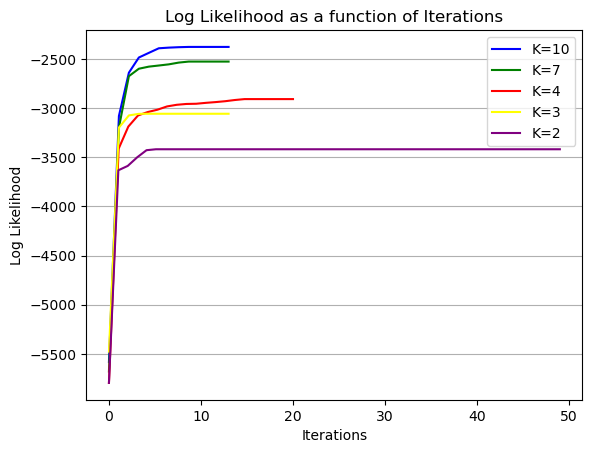
\includegraphics[width=0.7\textwidth]{images/image_3d.png}
    \caption{Log likelihood as a function of the number of iterations for K \in \{10,7,4,3,2\}} % Légende sous l'image
    \label{fig:image1} % Étiquette pour faire référence à l'image dans le texte
\end{figure}

We obtain the following parameters : 

For \( K = 10 \), we have
\[
\pi = \begin{bmatrix}
0.30035064 & 0.01 & 0.2199415 & 0.08970786 & 0.02 & 0.01 & 0.12063913 & 0.19936088 & 0.01 & 0.02
\end{bmatrix}
\]

For \( K = 7 \), we have
\[
\pi = \begin{bmatrix}
0.11070976 & 0.15 & 0.23000031 & 0.05999686 & 0.2400031 & 0.13929006 & 0.06999992
\end{bmatrix}
\]

For \( K = 4 \), we have
\[
\pi = \begin{bmatrix}
0.09999999 & 0.08 & 0.42000426 & 0.39999575
\end{bmatrix}
\]

For \( K = 3 \), we have
\[
\pi = \begin{bmatrix}
0.3402903 & 0.32979532 & 0.32991438
\end{bmatrix}
\]

For \( K = 2 \), we have
\[
\pi = \begin{bmatrix}
0.63116643 & 0.36883357
\end{bmatrix}
\]
\\

 \item e)

 In order to run the algorithm a few times starting from randomly chosen initial conditions, we used the code below, and obtained the following results :  \\

\begin{lstlisting}[language=Python, basicstyle=\ttfamily\small, frame=single, breaklines=true]
#We will there write commands to run the algorithm a 
# few times starting from randomly chosen initial conditions


def plot_various_K(obj,list=[2,3,4,7,10]):
    # This function allows us to plot on the same graph
    # the various simulations of the algorithm  
    # with random initial conditions

    R_list, P_List, Pi_List=[], [], []
    for a in list : 
        #We use our EM function to generate 
        # the results of the EM algorithm
        R, P, pi, y1=EM(a, X, 100, 1e-15)
        R_list.append(R)
        P_List.append(P)
        Pi_List.append(pi)
        x1 = np.linspace(0, len(y1), len(y1))
        obj.plot(x1, y1, label='K='+str(a))
    
    #We define labels and titles for our graphs
    obj.set_xlabel('Iterations')
    obj.set_ylabel('Log Likelihood')
    obj.grid(axis = "y")
    obj.set_title('Log Likelihood as a function of the number of Iterations')
    obj.legend() 

    return R_list, P_List, Pi_List

# We instanciate our multiple graphs
fig, axs = plt.subplots(3, 3, figsize=(24, 24))

#We generate the graphs of the multiple simulations of our EM algorithm
for k in range(axs.shape[0]):
    for j in range(axs.shape[1]):
        R_list, P_List, Pi_List = plot_various_K(axs[k][j])
        #print("R_list for iteration", k+j+1," : ", R_list)
        #print("P_list for iteration", k+j+1," : ", P_List)
        #print("Pi_list for iteration", k+j+1," : ", Pi_List)

plt.show()
\end{lstlisting}

\begin{figure}[H] % Position de l'image : 'h!' tente de placer l'image ici
    \centering % Centrage de l'image
    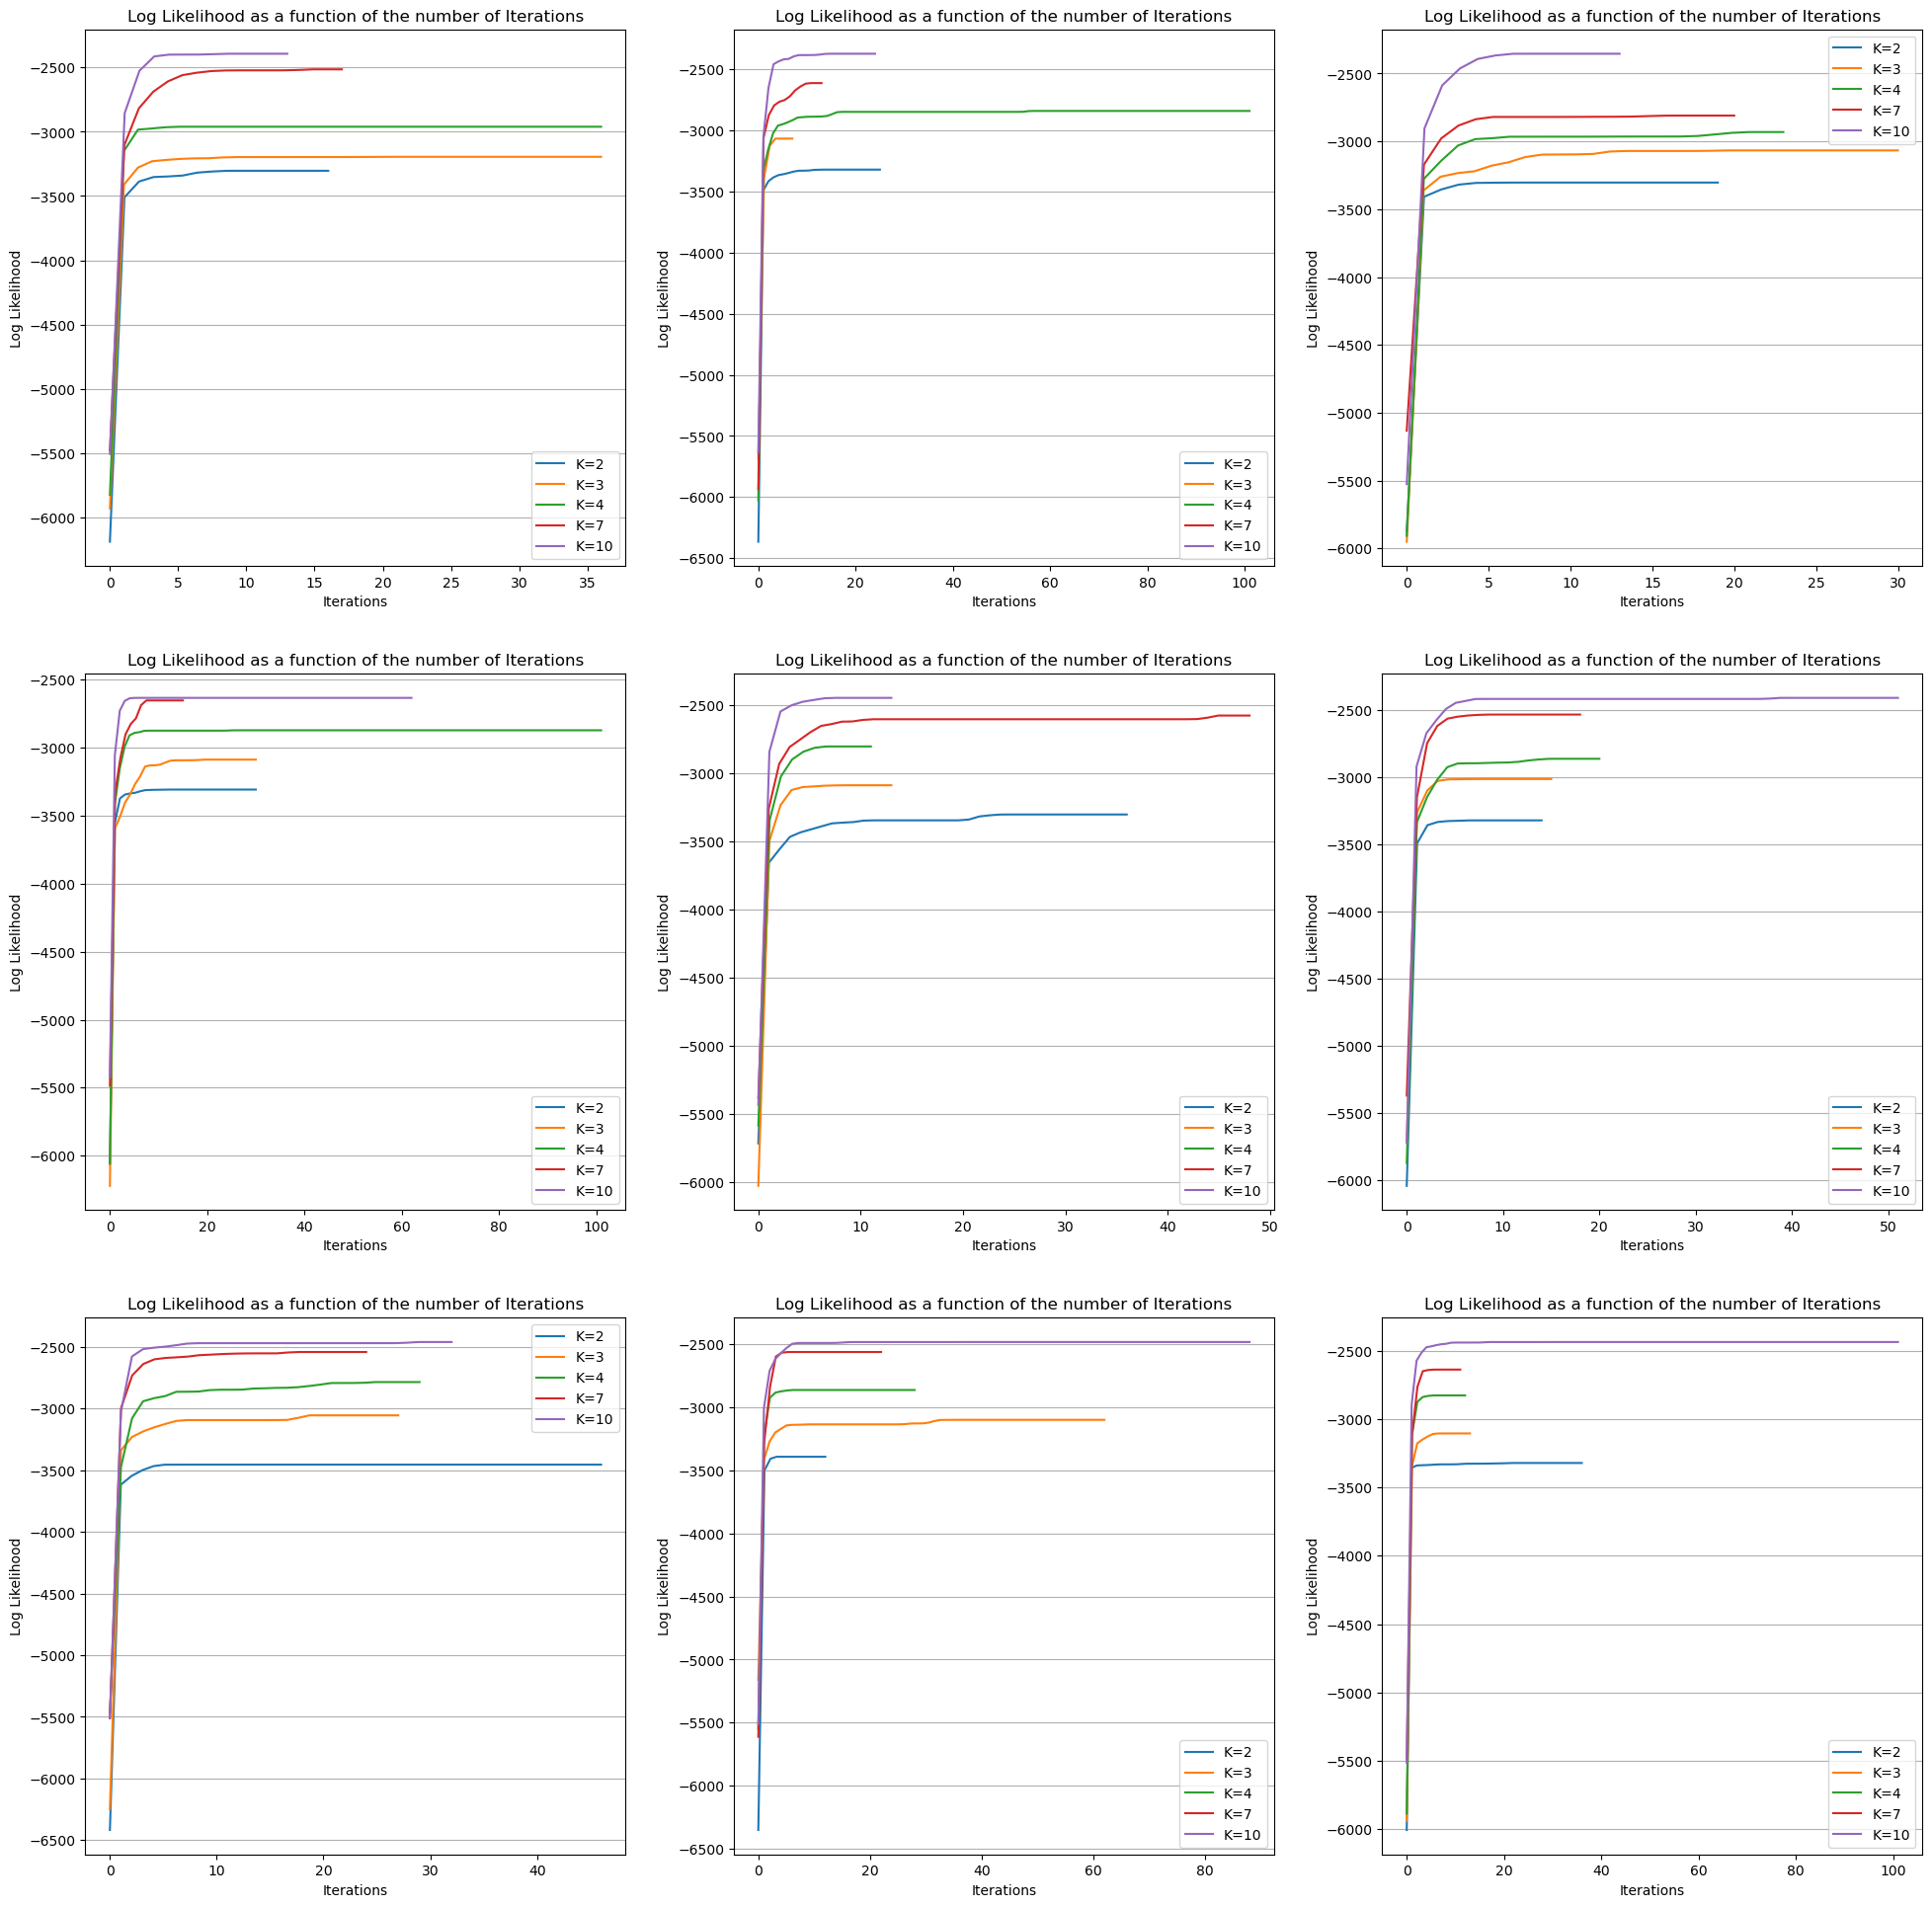
\includegraphics[width=0.9\textwidth]{images/image_3e.png}
    \caption{Multiple simulations of the Log likelihood as a function of the number of iterations for K \in \{10,7,4,3,2\}} % Légende sous l'image
    \label{fig:image1} % Étiquette pour faire référence à l'image dans le texte
\end{figure}
\\

We used the following code to plot our P matrices as images, and obtained the following result. On the image shown, you'll notice that the first line correspond to the 2 clusters found for K=2, the second line corresponds to the 3 clusters found for K=3, etc.

\begin{lstlisting}[language=Python, basicstyle=\ttfamily\small, frame=single, breaklines=true]
# We used this code to plot our P matrices as images

#We instanciate our graph
plt.figure()
fig, axs = plt.subplots(5, 10, figsize=(24, 24))

#We plot our P matrices as images in the instanciated graph
for k in range (np.shape(P_List)[0]):
    for l in range (np.shape(P_List[k])[0]):
        axs[k][l].imshow(np.reshape(P_List[k][l], (8,8)),interpolation="None",cmap='gray')

plt.axis('off')
plt.show()
\end{lstlisting}

\begin{figure}[H] % Position de l'image : 'h!' tente de placer l'image ici
    \centering % Centrage de l'image
    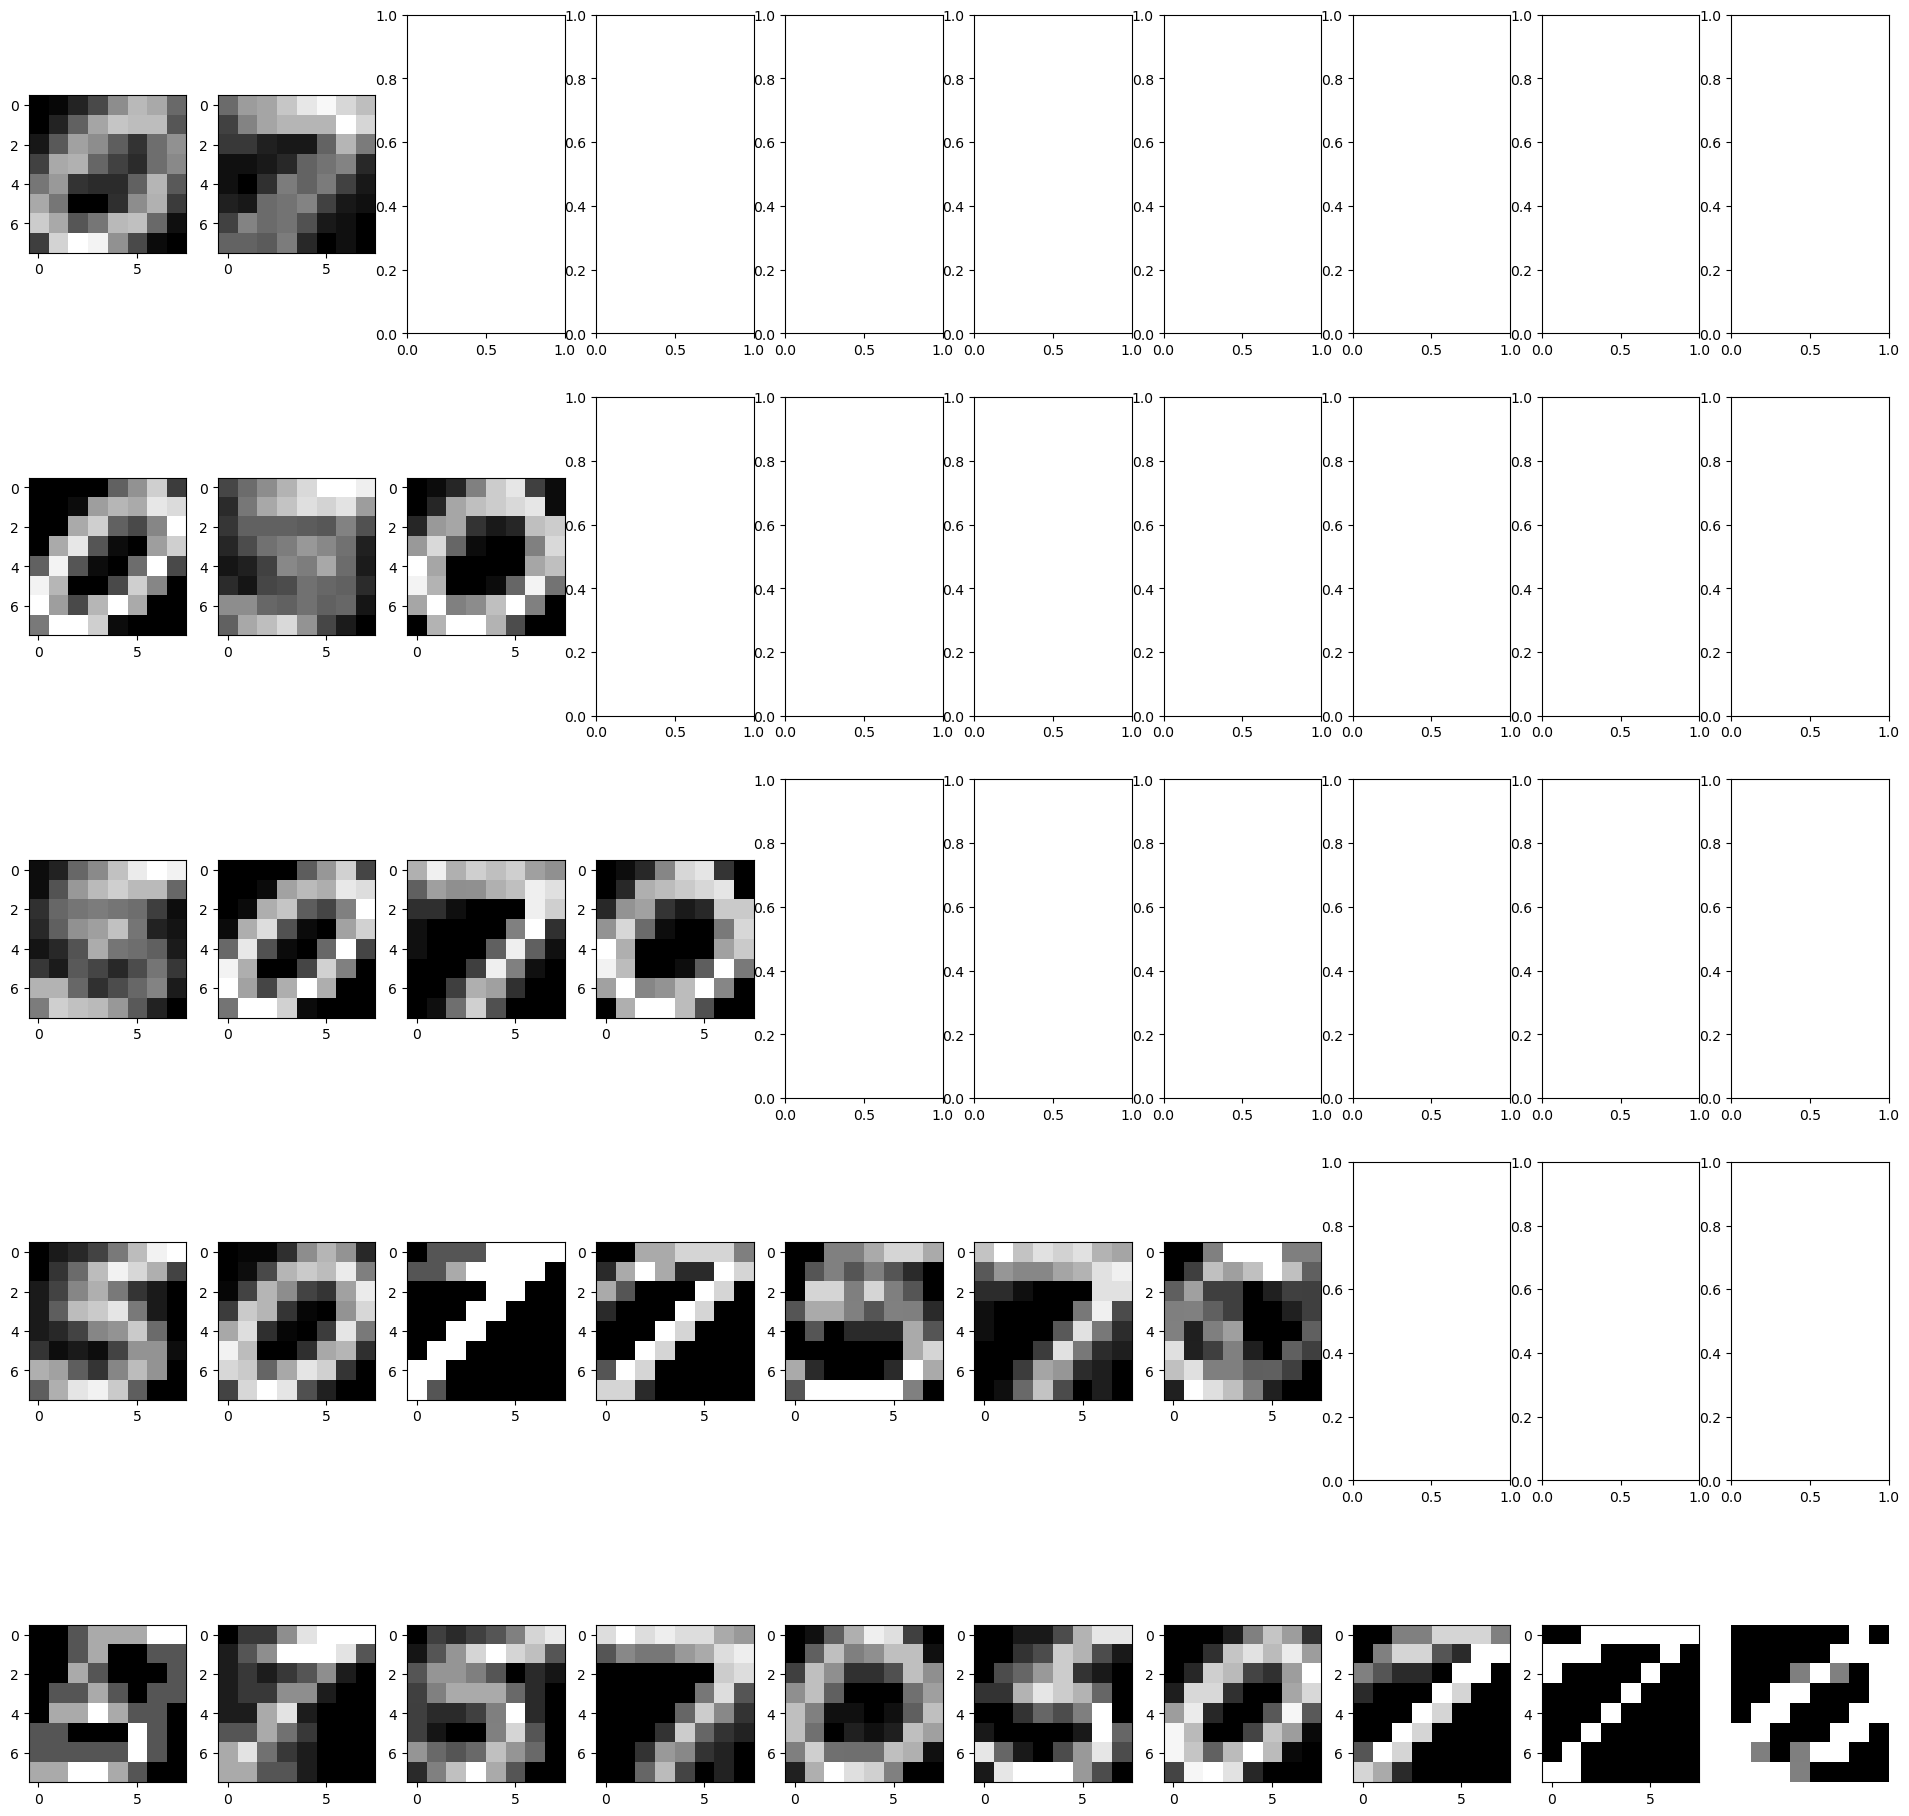
\includegraphics[width=0.9\textwidth]{images/image_3e2.png}
    \caption{Images of the clusters found for  K \in \{10,7,4,3,2\}} % Légende sous l'image
    \label{fig:image1} % Étiquette pour faire référence à l'image dans le texte
\end{figure}
\\

We observe that the more clusters we have, the bigger our log likelihood is. The hierarchy between the values of K seems to be the same on all of the simulations. Moreover, for a fixed value of K, the log likelihood seems to converge towards the same value every time we plot the algorithm.\\

Our algorithm seems to work, when we inspect our responsibility matrices, we notice that most of their lines are composed of "0" except for one "1" value. It means that our algorithm managed to assign our data to clusters with a high certainty. \\

Nevertheless, when we look at the images we plotted, we notice that, for high values of K, our algorithm map various clusters to the same number. Our algorithm is probably over-fitting for values of K that are too high. Similarly, our algorithm fails to detect some number for small values of K (we fail detect 5 for K=2, we fail to detect 7 for K=3). \\

To improve the model, I'd first suggest to select wisely the value of K. As our data is composed of 0, 5 and 7, I'd suggest selecting K superior to 3. Looking at the pictures shown, I'd probably select K=4 or K=7 as they seem to include all the numbers of the dataset (0,5,7). To choose K even more wisely, we would need information the different ways people write digits. If we have a dataset composed of ones, twos and threes, and if we know that people write the number one either like this "1" or like that "|", we could sugest to define 4 clusters, two for the two different ways of writing number one, one for number 2 and one for number 3.\\

\item f)\\

Expressed in bits, the log likelihood have 32 digits. Expressed naively, our data have N*D = 100*64 = 6400 bits. \\

A compression algorithm like gzip would surely allow to efficiently reduce the size of our data, as it would be easy to find similarities and patterns within our black and white images. Our log likelihood represents the amount of information that is needed to describe the data under the model, and is therefore an upper bound for the size of the data compressed with gzip.\\

\item g)\\

To encode matrix P with coefficients of 32 bits, we would need to use K*D*32 bits of space. \\

To encode the responsibility matrix with coefficients of 32 bits, we would need K*32 bits of space.\\

To encode our data, we would need D*N = 64*100=6400 bits.\\

Therefore, we would need D*N + 32*K + 32*K*D bits to store our data and the parameters of our model. Using gzip here might here be less efficient than the previous case in which we only had to compress our black and white images : it will be more difficult to find similarities in the data composed of the parameters of the model and of the images than to find similarities in the data composed only of the black and white images.\\ 

Finally, we can notice that the size of our model is linearly dependent on K. Hence, if K increases, the storage needed for our data increases. This information tells us that we should be careful when deciding about the complexity of our model : increasing the number of clusters that we want to find will not only increase the computation time, but will also increase the storage needed for our model.\\




% Section 4
\chapter{Exercise 4}

\item a)\\

We used the following code and obtained the following results. \\

When comparing the two graph obtained for latent state estimates, we notice that the smoothed graph is more smooth and "continuous", while the filtered graph is less "continuous" and more jagged. This is explained by the fact that filtering only involves predicting values of states estimates using past information, while smoothing uses both past information (past state estimates) and future information (observed data) to predict each of the values. We can notice that the "jagged" property of the filtered states estimates is even more visible at the beginning of the graph, when few historical data is available to predict the state estimates.\\

When comparing the two graphs obtained for the log determinant of covariance matrices, we notice that our logdet(V) do not converge towards the same value. This is explained, again, by the fact that the estimates obtained by filtering are generated only using the historical values of the latent state variables, while the estimates obtained by filtering are generated using past and future information. Hence, we are more confident about the values of the estimates obtained by smoothing (as we use past and future data, we have more information to compute them), which implies that their variance is less important. We can also notice that for the very last iterations, the value of logdet(V) of the smoothed estimates reaches the value of logdet(V) of the filtered estimates, which is explained by the fact that for the last iterations, the estimates obtained by smoothing are only calculated using past information (because there is no more future information), exactly like the estimates obtained by filtering. \\



\begin{lstlisting}[language=Python, basicstyle=\ttfamily\small, frame=single, breaklines=true]

# -*- coding: utf-8 -*-

"""
    File name: ssm_kalman.py
    Description: a re-implementation of the Kalman filter for http://www.gatsby.ucl.ac.uk/teaching/courses/ml1
    Author: Roman Pogodin / Maneesh Sahani (matlab version)
    Date created: October 2018
    Python version: 3.6
"""


import numpy as np
import matplotlib.pyplot as plt


def run_ssm_kalman(X, y_init, Q_init, A, Q, C, R, mode='smooth'):
    """
    Calculates kalman-smoother estimates of SSM state posterior.
    :param X:       data, [d, t_max] numpy array
    :param y_init:  initial latent state, [k,] numpy array
    :param Q_init:  initial variance, [k, k] numpy array
    :param A:       latent dynamics matrix, [k, k] numpy array
    :param Q:       innovariations covariance matrix, [k, k] numpy array
    :param C:       output loading matrix, [d, k] numpy array
    :param R:       output noise matrix, [d, d] numpy array
    :param mode:    'forw' or 'filt' for forward filtering, 'smooth' for also backward filtering
    :return:
    y_hat:      posterior mean estimates, [k, t_max] numpy array
    V_hat:      posterior variances on y_t, [t_max, k, k] numpy array
    V_joint:    posterior covariances between y_{t+1}, y_t, [t_max, k, k] numpy array
    likelihood: conditional log-likelihoods log(p(x_t|x_{1:t-1})), [t_max,] numpy array
    """
    d, k = C.shape
    t_max = X.shape[1]

    # dimension checks
    assert np.all(X.shape == (d, t_max)), "Shape of X must be (%d, %d), %s provided" % (d, t_max, X.shape)
    assert np.all(y_init.shape == (k,)), "Shape of y_init must be (%d,), %s provided" % (k, y_init.shape)
    assert np.all(Q_init.shape == (k, k)), "Shape of Q_init must be (%d, %d), %s provided" % (k, k, Q_init.shape)
    assert np.all(A.shape == (k, k)), "Shape of A must be (%d, %d), %s provided" % (k, k, A.shape)
    assert np.all(Q.shape == (k, k)), "Shape of Q must be (%d, %d), %s provided" % (k, k, Q.shape)
    assert np.all(C.shape == (d, k)), "Shape of C must be (%d, %d), %s provided" % (d, k, C.shape)
    assert np.all(R.shape == (d, d)), "Shape of R must be (%d, %d), %s provided" % (d, k, R.shape)

    y_filt = np.zeros((k, t_max))  # filtering estimate: \hat(y)_t^t
    V_filt = np.zeros((t_max, k, k))  # filtering variance: \hat(V)_t^t
    y_hat = np.zeros((k, t_max))  # smoothing estimate: \hat(y)_t^T
    V_hat = np.zeros((t_max, k, k))  # smoothing variance: \hat(V)_t^T
    K = np.zeros((t_max, k, X.shape[0]))  # Kalman gain
    J = np.zeros((t_max, k, k))  # smoothing gain
    likelihood = np.zeros(t_max)  # conditional log-likelihood: p(x_t|x_{1:t-1})

    I_k = np.eye(k)

    # forward pass

    V_pred = Q_init
    y_pred = y_init

    for t in range(t_max):
        x_pred_err = X[:, t] - C.dot(y_pred)
        V_x_pred = C.dot(V_pred.dot(C.T)) + R
        V_x_pred_inv = np.linalg.inv(V_x_pred)
        likelihood[t] = -0.5 * (np.linalg.slogdet(2 * np.pi * (V_x_pred))[1] +
                                x_pred_err.T.dot(V_x_pred_inv).dot(x_pred_err))

        K[t] = V_pred.dot(C.T).dot(V_x_pred_inv)

        y_filt[:, t] = y_pred + K[t].dot(x_pred_err)
        V_filt[t] = V_pred - K[t].dot(C).dot(V_pred)

        # symmetrise the variance to avoid numerical drift
        V_filt[t] = (V_filt[t] + V_filt[t].T) / 2.0

        y_pred = A.dot(y_filt[:, t])
        V_pred = A.dot(V_filt[t]).dot(A.T) + Q

    # backward pass

    if mode == 'filt' or mode == 'forw':
        # skip if filtering/forward pass only
        y_hat = y_filt
        V_hat = V_filt
        V_joint = None
    else:
        V_joint = np.zeros_like(V_filt)
        y_hat[:, -1] = y_filt[:, -1]
        V_hat[-1] = V_filt[-1]

        for t in range(t_max - 2, -1, -1):
            J[t] = V_filt[t].dot(A.T).dot(np.linalg.inv(A.dot(V_filt[t]).dot(A.T) + Q))
            y_hat[:, t] = y_filt[:, t] + J[t].dot((y_hat[:, t + 1] - A.dot(y_filt[:, t])))
            V_hat[t] = V_filt[t] + J[t].dot(V_hat[t + 1] - A.dot(V_filt[t]).dot(A.T) - Q).dot(J[t].T)

        V_joint[-2] = (I_k - K[-1].dot(C)).dot(A).dot(V_filt[-2])

        for t in range(t_max - 3, -1, -1):
            V_joint[t] = V_filt[t + 1].dot(J[t].T) + J[t + 1].dot(V_joint[t + 1] - A.dot(V_filt[t + 1])).dot(J[t].T)

    return y_hat, V_hat, V_joint, likelihood

#We define here our input variables

X = np.loadtxt('ssm_spins.txt')

A = 0.99 * np.array([
    [np.cos(2 * np.pi / 180), -np.sin(2 * np.pi / 180), 0, 0],
    [np.sin(2 * np.pi / 180), np.cos(2 * np.pi / 180), 0, 0],
    [0, 0, np.cos(2 * np.pi / 90), -np.sin(2 * np.pi / 90)],
    [0, 0, np.sin(2 * np.pi / 90), np.cos(2 * np.pi / 90)]])

Q = np.eye(4) - A @ A.T

Q0=np.ones((4,4))

C = np.array([
    [1, 0, 1, 0],
    [0, 1, 0, 1],
    [0, 0, 1, 0],
    [0, 0, 1, 1],
    [0.5, 0.5, 0.5, 0.5]])

R = np.eye(5)

Y0 = np.random.normal(loc=0, scale=1, size=(4,))

def is_positive_definite(A):
    """Check if matrix A is positive definite."""
    try:
        np.linalg.cholesky(A)
        return True
    except np.linalg.LinAlgError:
        return False

def logdet(A):
    """Compute the log-determinant of a matrix A, handling non-positive definite cases."""
    try:
        # Attempt Cholesky decomposition
        L = np.linalg.cholesky(A)
        return 2 * np.sum(np.log(np.diag(L)))
    except np.linalg.LinAlgError:
        # If not positive definite, add a small constant to the diagonal
        A += np.eye(A.shape[0]) * 1e-6
        L = np.linalg.cholesky(A)
        return 2 * np.sum(np.log(np.diag(L)))


# Run ssm_kalman function with 'filt' option
Y, V, _, L = run_ssm_kalman(X.T, Y0, Q0, A, Q, C, R, 'filt')

# Plot Y
plt.figure()
plt.plot(Y.T)
plt.title("Filtered State Estimates")
plt.xlabel("Time")
plt.ylabel("State Value")
plt.show()

# Plot log-determinants of V (covariance matrices)
logdet_values_filt = [logdet(v) for v in V]
plt.figure()
plt.plot(logdet_values_filt)
plt.title("Log-Determinant of Covariance Matrices (Filtered)")
plt.xlabel("Time")
plt.ylabel("logdet(V)")
plt.show()

# Run ssm_kalman function with 'smooth' option
Y, V, Vj, L = run_ssm_kalman(X.T, Y0, Q0, A, Q, C, R, 'smooth')

# Plot Y
plt.figure()
plt.plot(Y.T)
plt.title("Smoothed State Estimates")
plt.xlabel("Time")
plt.ylabel("State Value")
plt.show()

# Plot log-determinants of V (smoothed covariance matrices)
logdet_values_smooth = [logdet(v) for v in V]
plt.figure()
plt.plot(logdet_values_smooth)
plt.title("Log-Determinant of Covariance Matrices (Smoothed)")
plt.xlabel("Time")
plt.ylabel("logdet(V)")
plt.show()

\end{lstlisting} \\

\begin{figure}[H] % Position de l'image : 'h!' tente de placer l'image ici
    \centering % Centrage de l'image
    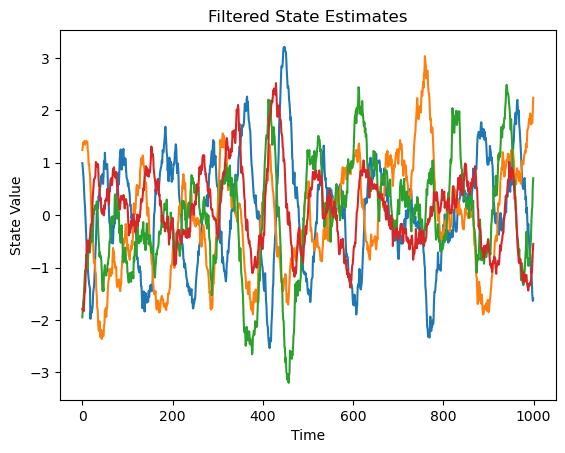
\includegraphics[width=0.5\textwidth]{images/image_4a1.png}
    \caption{Visualization of filtered states estimates over time} % Légende sous l'image
    \label{fig:image1} % Étiquette pour faire référence à l'image dans le texte
\end{figure} \\

\begin{figure}[H] % Position de l'image : 'h!' tente de placer l'image ici
    \centering % Centrage de l'image
    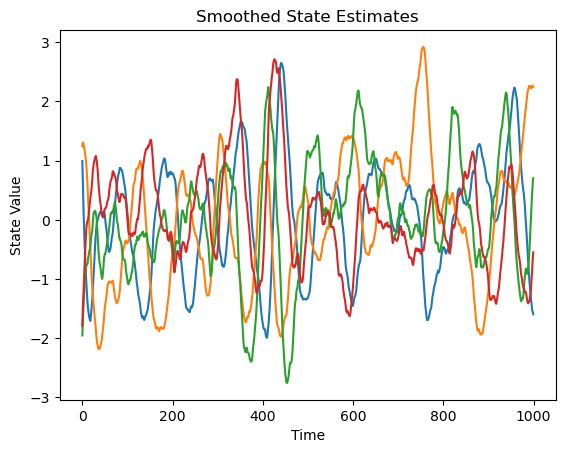
\includegraphics[width=0.5\textwidth]{images/image_4a3.png}
    \caption{Visualization of smoothed states estimates over time} % Légende sous l'image
    \label{fig:image1} % Étiquette pour faire référence à l'image dans le texte
\end{figure} \\

\begin{figure}[H] % Position de l'image : 'h!' tente de placer l'image ici
    \centering % Centrage de l'image
    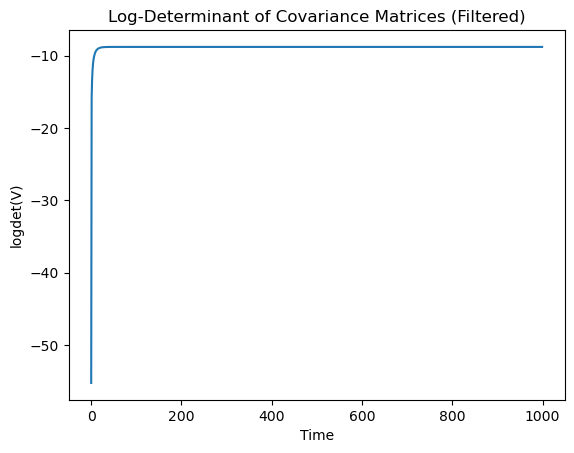
\includegraphics[width=0.5\textwidth]{images/image_4a2.png}
    \caption{Visualization of log determinant of the covariances matrices over time (filtered)} % Légende sous l'image
    \label{fig:image1} % Étiquette pour faire référence à l'image dans le texte
\end{figure} \\

\begin{figure}[H] % Position de l'image : 'h!' tente de placer l'image ici
    \centering % Centrage de l'image
    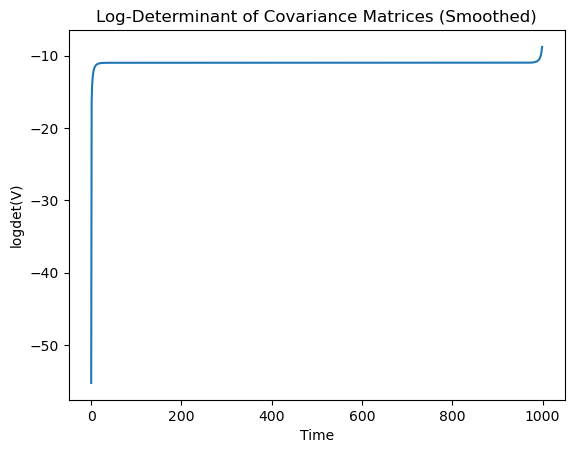
\includegraphics[width=0.5\textwidth]{images/image_4a4.png}
    \caption{Visualization of log determinant of the covariances matrices over time (smoothed)} % Légende sous l'image
    \label{fig:image1} % Étiquette pour faire référence à l'image dans le texte
\end{figure} \\

\item b)\\

In the lecture, we determined that : \\

\[
C_{new} = \big(\sum_t x_t\langle y_t \rangle ^T \big)  \big(\sum_t \langle y_ty_t^T \rangle \big)^{-1}
\]
\[
A_{new} = \big(\sum_t \langle y_{t+1}y_t^T \rangle \big)  \big(\sum_t \langle y_ty_t^T \rangle \big)^{-1}
\]


% Section 5
\chapter{Exercise 5}

\item a)

Let's write $N_{\alpha, \beta}$, the number of times the transition $\alpha, \beta$ happens. \\

We have therefore $\underset{{\beta}}\sum \psi_{\alpha, \beta} = 1$ \\

We can then write $p(s_1, ..., s_n) = p(s_1)\Pi_{i=2}^n p(s_i|s_{i-1}) = p(s_1) \underset{{\alpha, \beta}}\Pi \psi(\alpha, \beta) =p(s_1)\underset{{\alpha, \beta}}\Pi \psi(\alpha, \beta)^{N_{\alpha, \beta}}$ \\

We want to solve the following optimization problem (O) : \\

\[ (O) \Leftrightarrow
 \left\{
\begin{array}{l}
\text{$\underset{{\alpha, \beta}}{argmax} \underset{{\alpha, \beta}}\Pi \psi(\alpha, \beta) = \underset{{\alpha, \beta}}{argmax} log(p(s_1)) + \underset{{\alpha, \beta}}\sum N_{\alpha, \beta} log(\psi(\alpha, \beta))$} \\
\text{so that}\\
\text{$\underset{{\beta}}\sum \psi_{\alpha, \beta} = 1$}
\end{array}
\right.
\] \\

\[ (O) \Leftrightarrow
 \left\{
\begin{array}{l}
\text{$\frac{\partial}{\partial \psi(\alpha, \beta)}(log\big(p(s_1)) +  \underset{{\alpha, \beta}}\sum N_{\alpha, \beta} log(\psi(\alpha, \beta)) + \lambda (\underset{{\beta}}\sum \psi_{\alpha, \beta} - 1)\big) = 0$} \\
\text{$\underset{{\beta}}\sum \psi_{\alpha, \beta} = 1$}
\end{array}
\right.
\] \\

\[ (O) \Leftrightarrow
 \left\{
\begin{array}{l}
\text{$\frac{N_{\alpha, \beta}}{\psi(\alpha,\beta)} - \lambda=0$} \\
\text{$\underset{{\beta}}\sum \psi_{\alpha, \beta} = 1$}
\end{array}
\right.
\] \\

\[ (O) \Leftrightarrow
 \left\{
\begin{array}{l}
\text{$\frac{N_{\alpha, \beta}}{\psi(\alpha,\beta)} - \lambda=0$} \\
\text{$\frac{N_{\alpha, \beta}}{\psi(\alpha,\beta)} = \lambda$} \\
\text{$\underset{{\beta}}\sum \psi_{\alpha, \beta} = 1$}
\end{array}
\right.
\] \\

\[ (O) \Leftrightarrow
 \left\{
\begin{array}{l}
\text{$\frac{N_{\alpha, \beta}}{\psi(\alpha,\beta)} - \lambda=0$} \\
\text{$\underset{\beta}\sum N_{\alpha, \beta} = \lambda \underset{\beta}\sum\psi(\alpha, \beta)$} \\
\text{$\underset{{\beta}}\sum \psi_{\alpha, \beta} = 1$}
\end{array}
\right.
\] \\

\[ (O) \Leftrightarrow
 \left\{
\begin{array}{l}
\text{$\frac{N_{\alpha, \beta}}{\psi(\alpha,\beta)} - \lambda=0$} \\
\text{$\underset{\beta}\sum N_{\alpha, \beta} = \lambda$} \\
\text{$\underset{{\beta}}\sum \psi_{\alpha, \beta} = 1$}
\end{array}
\right.
\] \\

\[ (O) \Leftrightarrow
 \left\{
\begin{array}{l}
\text{$\frac{N_{\alpha, \beta}}{\underset{\beta}\sum N_{\alpha, \beta}} = \psi(\alpha,\beta)$} \\
\text{$\underset{{\beta}}\sum \psi_{\alpha, \beta} = 1$}
\end{array}
\right.
\] \\

Therefore, the solution is given by $\psi(\alpha,\beta)=\frac{N_{\alpha, \beta}}{\underset{\beta}\sum N_{\alpha, \beta}} $ \\

To compute the transition matrix and the stationary matrix, we used the code below and obtained the  following results : 

\begin{lstlisting}[language=Python, basicstyle=\ttfamily\small, frame=single, breaklines=true]
# We import the provided data

war_and_peace = open("war_and_peace.txt", "r").read()
war_and_peace = war_and_peace.replace("\n", "").lower()

symbols = open("symbols.txt", "r").read()
symbols = symbols.replace("\n", "")

encrypted_message = open("message.txt", "r").read()

def transition_mat(text, symbols):
    #This function computes the transition matrix
    matrix = np.zeros(shape=(len(symbols),len(symbols)))

    for i in range(len(text)):
        if text[i-1] in symbols and text[i] in symbols:
            beta, alpha = symbols.index(text[i-1]), symbols.index(text[i])
            matrix[alpha][beta] += 1
        else:
            continue

    transition_matrix = np.zeros((len(symbols),len(symbols)))
    for i in range(len(symbols)):
        # We divide every coefficient of each column by the sum of 
        # the coefficients of the column to ensure that each column sum to 1
        transition_matrix[i,:] = matrix[i,:]/(np.sum(matrix,axis=1)[i])

    return transition_matrix

# We plot our transition matrix as a heatmap

plt.figure(figsize=(12, 12))  # Taille de la figure
sns.heatmap(transition_mat(war_and_peace,symbols), cmap="YlGnBu", 
            cbar=True, cbar_kws={'label': 'Probability of transition'}, 
            xticklabels=symbols, yticklabels=symbols)
plt.title("Heatmap showing the transition probabilities")
plt.show()

def Stationary_Distributions(text):
    #This function computes the stationary distribution matrix

    stationary_distribution = np.zeros((1,len(symbols)))
    
    for i in range(len(text)):
        if text[i] in symbols:
            index = symbols.index(text[i])
            stationary_distribution[0][index] += 1
        else:
            continue

    stationary_stistribution_final = np.zeros((1,len(symbols)))
    for i in range(len(symbols)):
        # We divide every coefficient of our matrix by the sum of 
        # the coefficients of the matrix to ensure that the coefficients sum to 1
        stationary_stistribution_final[0][i] = stationary_distribution[0][i]/(np.sum(stationary_distribution[0]))

    return stationary_stistribution_final

# We plot our stationary distribution matrix as a heatmap

plt.figure(figsize=(20, 2))
sns.heatmap(Stationary_Distributions(war_and_peace), cmap="YlGnBu", 
            cbar=True, cbar_kws={'label': 'Probability of transition'}, 
            xticklabels=symbols)
plt.title("Heatmap showing the stationary distribution of symbols")
plt.show()

\end{lstlisting}

\begin{figure}[H] % Position de l'image : 'h!' tente de placer l'image ici
    \centering % Centrage de l'image
    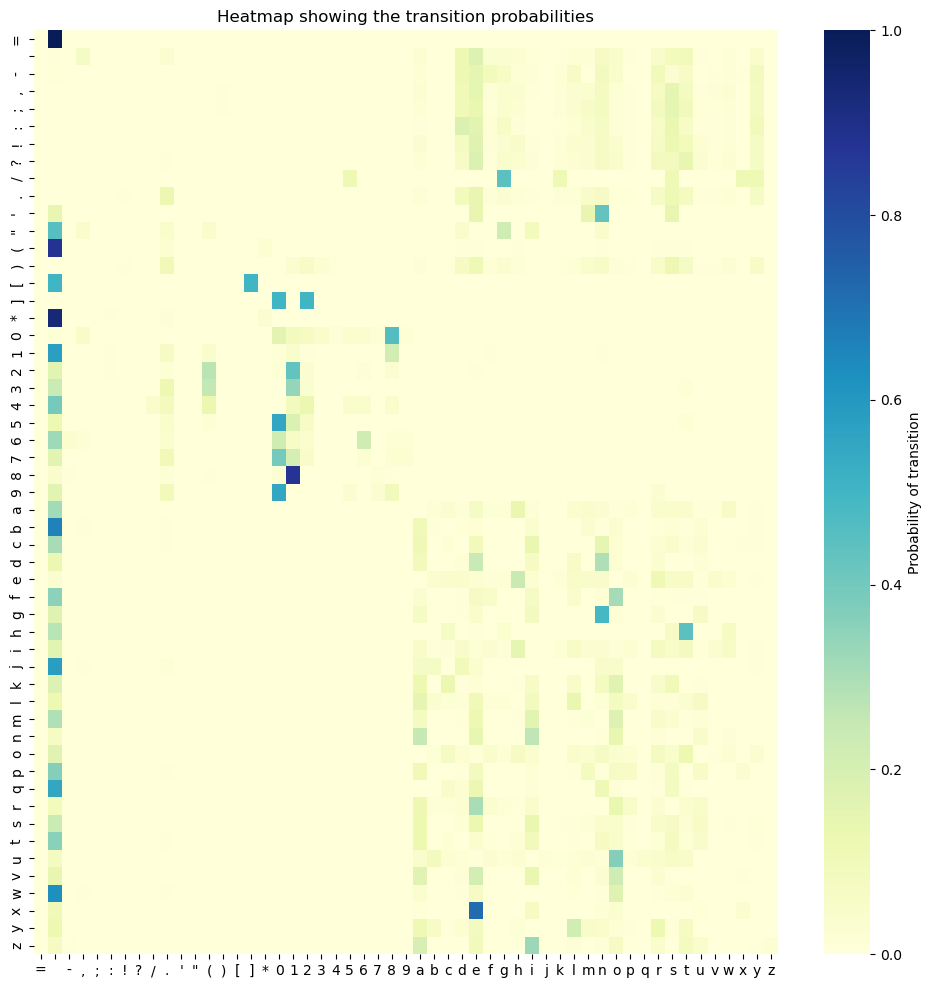
\includegraphics[width=0.9\textwidth]{images/image_5b1.png}
    \caption{Heatmap showing the transition matrix} % Légende sous l'image
    \label{fig:image1} % Étiquette pour faire référence à l'image dans le texte
\end{figure}

\begin{figure}[H] % Position de l'image : 'h!' tente de placer l'image ici
    \centering % Centrage de l'image
    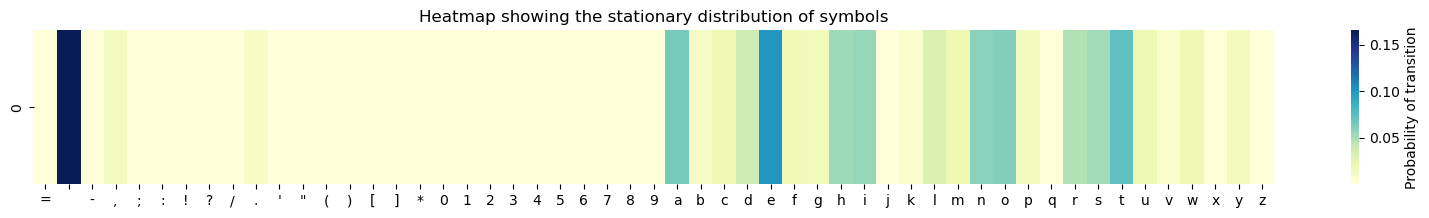
\includegraphics[width=0.9\textwidth]{images/image_5b2.png}
    \caption{Heatmap showing the stationary probabilities matrix} % Légende sous l'image
    \label{fig:image1} % Étiquette pour faire référence à l'image dans le texte
\end{figure}


\item b)

The mapping between symbols is one-to-one. Therefore, for $a\neq a'$, if $\sigma(a) = b$, there is no possibility that $\sigma(a') = b$. Hence, $P(\sigma(a) = b \vert \sigma(a') = b')$ is different from $P(\sigma(a)=b)$.\\

Let us write : $\forall i \in {1,..,n}, \sigma(e_i) = k_i$ \\

We have : \\

\[
P(e_1, ..., e_n \vert \sigma) = P\big(e_1, ..., e_n \vert \sigma(k_1) = e_1, ..., \sigma(k_n) = e_n\big) 
\] \\

\[ \implies
P(e_1, ..., e_n \vert \sigma) = P(k_1, ..., k_n) 
\] \\

\[ \implies
P(e_1, ..., e_n \vert \sigma) = P(k_1)\times \prod_{i=2}^{n}\Psi(k_i, k_{i-1}) 
\] \\

\[ \implies
P(e_1, ..., e_n \vert \sigma) = \Phi(k_1) \times \Psi(k_i, k_{i-1})
\] \\

\item c)

If $\sigma$ and $\sigma'$ are different chains, we obtain $S(\sigma \rightarrow \sigma')$ by randomly choosing one of the symbols $s_1$, by choosing a second one $s_2$, and by swapping their encrypted value. We therefore have :
$
\\

\[ 
S(\sigma \rightarrow \sigma') = P(s_1)P_{s_1}(s_2)+P(s_2)P_{s_2}(s_1) \] \\
\[ \implies
S(\sigma \rightarrow \sigma') = \frac{1}{53}\frac{1}{52} + \frac{1}{53}\frac{1}{52} \] \\
\[ \implies
S(\sigma \rightarrow \sigma') = \frac{2}{53\times52}\] \\
Hence, $S(\sigma \rightarrow \sigma')$  is independent of $\sigma$ and $\sigma'$.
\\

As S is symmetric, we have $S(\sigma \rightarrow \sigma') = S(\sigma' \rightarrow \sigma)$, which gives : \\
\[ 
A(\sigma \rightarrow \sigma') = min\big(1, \frac{S(\sigma \rightarrow \sigma') P(\sigma' \vert D')}{S(\sigma \rightarrow \sigma') P(\sigma \vert D)} \big)= min\big(1, \frac{ P(\sigma' \vert D')}{P(\sigma \vert D)} \big)
\] \\

If use Bayes Theorem and the expression of $P(e_1, ..., e_n \vert \sigma)$ found in the previous question, we can write : \\
\[ 
P(\sigma \vert D) = P(D \vert \sigma)\frac{P(\sigma)}{P(D)}= P(e_1, ..., e_n \vert \sigma)\frac{P(\sigma)}{P(D)}= \frac{P(\sigma)}{P(D)}\Phi(k_1)\prod_{i=2}^{n}\Psi(k_i, k_{i+1}) \] \\

Similarly, we find :
$
P(\sigma' \vert D) = \frac{P(\sigma')}{P(D)}\Phi(k'_1)\prod_{i=2}^{n}\Psi(k'_i, ,k'_{i + 1})
$ \\

We can rewrite A as : $
A(\sigma \rightarrow \sigma' \vert D) = min\big(1, \frac{P(\sigma')}{P(D)}\frac{P(D)}{P(\sigma')}\frac{\Phi(k'_1)\prod_{i=2}^{n}\Psi(k'_i, ,k'_{i + 1})}{\Phi(k_1)\prod_{i=2}^{n}\Psi(k_i, ,k_{i + 1})}\big)
$\\

Finally, as we have $P(\sigma)=P(\sigma')$, we can rewrite A as :\\
\[ 
A(\sigma \rightarrow \sigma' \vert D) = min\big(1, \frac{\Phi(k'_1)\prod_{i=2}^{n}\Psi(k'_i, ,k'_{i + 1})}{\Phi(k_1)\prod_{i=2}^{n}\Psi(k_i, ,k_{i + 1})}\big)
\] \\

\item d)

To implement the MH sampler, I used the code below and obtained the following results. In order for our algorithm to converge faster, we implemented an "intelligent" initialization for sigma.  We associated the k-th most probable symbol according to our stationary probabilities with the k-th most recurring symbol in our text. This initialization allows our algorithm to converge faster as it gives a plausible first value for sigma. \\

The table summarizing the obtained results for every 100 iterations is quite small as we have a lot of values to show, please forgive this inconvenience. In case you do not manage to read, I write here that we have a readable sentence ("in my younger and more vulnerable years my father gave me so") after 8300 iterations, and for a log likelihood of -3572.8.\\

\begin{lstlisting}[language=Python, basicstyle=\ttfamily\small, frame=single, breaklines=true]
def decrypt_message(encrypted_message, sigma):
    #This function decrypts the message using Sigma
    decripted_message = ''
    for letter in encrypted_message :
        decripted_message += symbols[sigma.index(letter)]
    return decripted_message

def loglikelihood(encrypted_message, stationary_distribution, sigma, transition_matrix):
    # This function computes the loglikelihood of the message decrypted using sigma
    decripted_message = decrypt_message(encrypted_message, sigma)
    log_likelihood = np.log(stationary_distribution[symbols.index(decripted_message[0])]+10**(-4))
    for k in range (0, len(encrypted_message)):
        alpha = symbols.index(decripted_message[k])
        beta = symbols.index(decripted_message[k-1])
        log_likelihood += np.log(transition_matrix[alpha][beta]+10**(-4))
    return log_likelihood

def mcmc_step(sigma, p_old, transition_matrix, stationary_distribution):
    #This function performs one MCMC step
    
    #Select two random symbols
    symbols_= sigma[:]
    proposal_1 = np.random.choice(symbols_)
    symbols_.remove(proposal_1)
    proposal_2 = np.random.choice(symbols_)

    #Get their respective indexes
    index1 = sigma.index(proposal_1)
    index2 = sigma.index(proposal_2)

    #Switch the indexes to create a new list of symbols, sigma_new
    sigma_new = sigma[:]
    sigma_new[index1], sigma_new[index2] = sigma_new[index2], sigma_new[index1]

    #Compute the new log likelihood
    p_new=loglikelihood(encrypted_message, stationary_distribution, list(sigma_new), transition_matrix)

    #Define the rejection kernel
    threshold=min(1,np.exp(p_new-p_old))
    
    #Accept or reject sigma_new
    if (p_new >= p_old) or (threshold >= np.random.uniform(0,1)):
        accepted=True
        #print(sigma_new)
        print(p_new)
        return sigma_new, accepted, p_new
    else:
        accepted=False
        return sigma, accepted, p_old
    
def run_mcmc(N_iters, sigma_init, p_old, transition_matrix, stationary_distribution):
    #This function runs the MCMC algorithm

    #We instanciate our variables
    sigma_chain = [sigma_init]
    p_old_chain=[p_old]
    N_accepted = 0
    data_for_report={"Number of iterations" : [], "Decrypted message" : [], "Loglikelihood" : []}

    #We run the algorithm
    for _ in range(N_iters):
        sigma, accepted, p_old = mcmc_step(sigma_chain[-1], p_old_chain[-1], transition_matrix, stationary_distribution)
        sigma_chain.append(sigma)
        p_old_chain.append(p_old)
        N_accepted += accepted

        #We capture our data every 100 iteration, for the report
        if _ % 100 ==0:
            data_for_report["Number of iterations"].append(_)
            data_for_report["Decrypted message"].append(decrypt_message(encrypted_message, list(sigma))[:60])
            data_for_report["Loglikelihood"].append(p_old)
        
    return np.stack(sigma_chain), np.stack(p_old_chain), N_accepted / N_iters, pd.DataFrame.from_dict(data_for_report)

def kth_largest_index(lst, k):
    #This function finds the index of the kth largent element in a list

    #Sort the list in descending order, keeping only unique values
    unique_sorted = sorted(set(lst), reverse=True)
    
    # Check if k is within the range of unique elements
    if k > len(unique_sorted) :
        raise ValueError("k is out of range for the number of unique elements in the list.")
    
    #Get the k-th largest element
    kth_largest_element = unique_sorted[k]
    
    #Find the index of the k-th largest element in the original list
    return list(lst).index(kth_largest_element)

def intelligent_initialization(sigma, stationary_distribution, encrypted_message):
    #This function performs an intelligent initialization. Its principle is explained in the report.
    
    sigma_new=sigma[:]

    for k in range (len(Counter(encrypted_message).most_common())) :
        print(k)
        #We extract the k most recurring symbol of our encripted message, and its index in our symbol list
        k_most_recurring_symbol_encrypted=Counter(encrypted_message).most_common()[k][0]
        index_k_most_recurring_symbol_encrypted=sigma.index(k_most_recurring_symbol_encrypted)
        print(k_most_recurring_symbol_encrypted)
        print(index_k_most_recurring_symbol_encrypted)
 
        #We extract the k most recurring symbol of our stationary distribution, and its index in our symbol list
        index_k_most_recurring_symbol_stationary=kth_largest_index(stationary_distribution, k)
        print(index_k_most_recurring_symbol_stationary)
        #index_k_most_recurring_symbol_stationary=sigma.index(k_most_recurring_symbol_stationary)

        #We assign the most k most recurring symbol of our encripted message to the k most recurring symbol of our stationary distribution
        sigma_new[index_k_most_recurring_symbol_stationary], sigma_new[index_k_most_recurring_symbol_encrypted] = sigma_new[index_k_most_recurring_symbol_encrypted], sigma_new[index_k_most_recurring_symbol_stationary]

    return sigma_new


# Here, we run the MCMC Algorithm

N_samples = 15000
transition_matrix=transition_mat(war_and_peace, symbols)
stationary_distribution=Stationary_Distributions(war_and_peace)[0]
p_old_init=loglikelihood(encrypted_message, stationary_distribution, list(symbols), transition_matrix)
initial_sigma=intelligent_initialization(list(symbols), stationary_distribution, encrypted_message)

sigma_chain, p_old_chain, accepted, data_for_report = run_mcmc(N_samples, initial_sigma, p_old_init, transition_matrix, stationary_distribution)
print("acceptance rate:", accepted)
print(decrypt_message(encrypted_message, list(sigma_chain[-1])))

\end{lstlisting}

\begin{figure}[H] % Position de l'image : 'h!' tente de placer l'image ici
    \centering % Centrage de l'image
    
\includegraphics[width=0.4\textwidth]{images/dataframe_image.png}
    \caption{Current decryption of the first 60 symbols after every 100 iterations} % Légende sous l'image
    \label{fig:image1} % Étiquette pour faire référence à l'image dans le texte
\end{figure}


\item e)

Some values $\Psi(\alpha, \beta)$ might be $0$. The chain is therefore not irreducible and thus not ergodic. To solve this problem, we could fill the $0$'s of our transition matrix with small values ($10^{-4}$ in the code). By doing that, we allow the chain to reach every possible state, and restore its ergodicity.

\item f)

Symbol probabilities alone would not sufficient because the text is specific and might contain an abnormal amount of an improbable letter, which would prevent us from finding the right distribution. Moreover, if we only use probabilities without taking the order into account, "aabbcc" is considered to be as likely as "ababcc". A model which only considers probabilities would therefore converge towards a chain containing the right symbols, but not in the right order. \\

A second order Markov chain could work, as it would increase the importance of the order of the letters. The drawback might be the computation time, which would be more important as we have a bigger transition matrix. We might also overfit our training data if its size is not sufficient.\\

Allowing two symbols to be mapped to the same encrypted symbol would not work : we would have to choose between the two possible values, which lead to the same problems that we mentioned with the "probabilistic only" approach before.\\ 

The method of this exercise would work with a Chinese text. Nevertheless, our transition matrix would be much larger and we would need a very important training set to compute accurate coefficients for our matrix, as we might end up otherwise with a transition matrix mostly composed of zeros, which would lead to non-accurate decryption results.\\


% Section 7
\chapter{Exercise 7}

\item a)

We have the following optimization problem (O) : 

\[
(O) \Leftrightarrow \left\{
\begin{array}{l}
\text{$\max_{x,y}$ f(x,y)} \\
\text{so that}\\
\text{g(x,y) = $y^2$ +xy -1 = 0}
\end{array}
\right.
\] \\


The solution of our problem is the solution of the system (S) : 

\[
(S) \Leftrightarrow \left\{
\begin{array}{l}
\text{$\nabla f$ + $\nabla g$ = 0} \\
\text{g(x,y)=0}
\end{array}
\right.
\] \\

\[
(S) \Leftrightarrow \left\{
\begin{array}{l}
\text{1 + $\lambda$ y = 0} \\
\text{2 + $\lambda$ (2y+x) = 0}\\
\text{$y^2$ + xy = 1}
\end{array}
\right.
\] \\

\[
(S) \Leftrightarrow \left\{
\begin{array}{l}
\text{$\lambda$ = $\frac{-1}{y}$, which is possible because y$\neq$0} \\
\text{2 + $\lambda$ (2y+x) = 0 $\implies \frac{-x}{y}$ = 0 $\implies x=0$ }\\
\text{$y^2$ + xy = 1}
\end{array}
\right.
\] \\

\[
(S) \Leftrightarrow \left\{
\begin{array}{l}
\text{$\lambda$ = 1 or $\lambda$ = -1} \\
\text{x = 0}\\
\text{y = 1 or y = -1}
\end{array}
\right.
\] \\
\vspace{0.5 cm}

In conclusion, the points (0, 1) and (0, -1) are local extremas of our function f. \\

\item b) i)

We know how to evaluate $e^x$. Therefore, if we are capable to find the value of $x^*$ which annulate f(x,a)= $e^x$  - a, we are able to evaluate ln(a) : 

\[
f(x^*,a) = 0 \Leftrightarrow e^{x^{*}} - a = 0 \Leftrightarrow x^*=ln(a)
\] \\

\item b) ii)

The generic equation of Newton's algorithm is :
\[
x_{n+1} = x_n + \frac{f(x_n)}{f'(x_{n})} = x_n + \frac{e^{x_n}-a}{e^{-x_n}} = x_n + 1 - ae^{x_n}
\] \\

% Section 8
\chapter{Exercise 8}

\item a)

We have $\sup_{x \in R^n} R_A(x) = \sup_{x \in R^n} \frac{x^TAx}{\|x\|^2} = \sup_{x \in R^n} \frac{x^T}{\|x\|}A\frac{x}{\|x\|}$ \\

We notice that $\| \frac{x^T}{\|x\|} \| =  \frac{\|x^T\|}{\|x\|} = \frac{\|x\|}{\|x\|} = 1$ \\

Therefore, if we write x' = $\frac{x}{\|x\|}$ for $x \in R^n$, we have : 
\[
\sup_{x \in R^n} R_A(x) = \sup_{x' \in S} R_A(x') = \sup_{x' \in S} x'^TAx = \sup_{x' \in S} R'_A(x')
\] \\

$R'_A$ is continuous on S, which is a compact. Thus, according to the extreme value theorem of calculus, $\sup_{x \in R^n} R_A(x) = \sup_{x' \in S} R'_A(x')$ is attained.\\

\item b)

Using the fact that $x=\sum_{i=1}^n (\xi_i^Tx)\xi_i$, we can rewrite $R_A(x)$ : 

\[
 R_A(x) =  \frac{x^TAx}{\|x\|^2} = \frac{x^T}{\|x\|^2} A \sum_{i=1}^n (\xi_i^Tx)\xi_i
\] \\

$(\xi_i^Tx)$ is a scalar and commutes with $\xi_i$, we have therefore : 

\[
 R_A(x) = \frac{x^T}{\|x\|^2} \sum_{i=1}^n A\xi_i(\xi_i^Tx) = \frac{x^T}{\|x\|^2} \sum_{i=1}^n \lambda_i\xi_i(\xi_i^Tx) = \frac{x^Tx}{\|x\|^2} \sum_{i=1}^n \lambda_i\xi_i\xi_i^T = \sum_{i=1}^n \lambda_i\xi_i\xi_i^T
\] \\

We recall that $\forall i  \in \( \llbracket 1, n \rrbracket \), \lambda_i \leq \lambda_1$, which gives : \\

\[
 R_A(x)  \leq \lambda_1 \sum_{i=1}^n \xi_i\xi_i^T
\] \\

Finally, the fact that vectors $\xi_i$ form an ONB, leads to  $\sum_{i=1}^N\xi_i\xi_i^T = 1$ and gives the final result : \\

\[
 R_A(x)  \leq \lambda_1
\] \\

\item c)

Let's assume that : $\exists x^* \in R^n /x^*$ is not contained in span $\{\xi_1, ..., \xi_k\}$\\

We can then write $x^*=\sum_{l=k+1}^n(\xi_l^tx)\xi_l$\\

Using the same demonstration as in question b), we obtain that : \\
\[
R_A(x^*) \leq \max_{l\in \llbracket k+1, n \rrbracket}(\lambda_l)
\] \\

We know that all the remaining eigenvectors $(\xi_l)_{l\in \llbracket k+1, n \rrbracket}$ have a distinct eigenvalue from $\lambda_1$, and that their respective eigenvalues are inferior or equal to $\lambda_1$. This result applies in particular to $\max_{l\in \llbracket k+1, n \rrbracket}(\lambda_l)$, which gives us the final result : \\

\[
R_A(x^*) \leq \max_{l\in \llbracket k+1, n \rrbracket}(\lambda_l) < \lambda_1
\] \\

\end{document}
